\chapter{Application Design}
\label{appendix:design}

The Figures provided on the following pages are screenshots from the later phases of the development of the final prototype.

\begin{figure}[ht!]
    \centering
    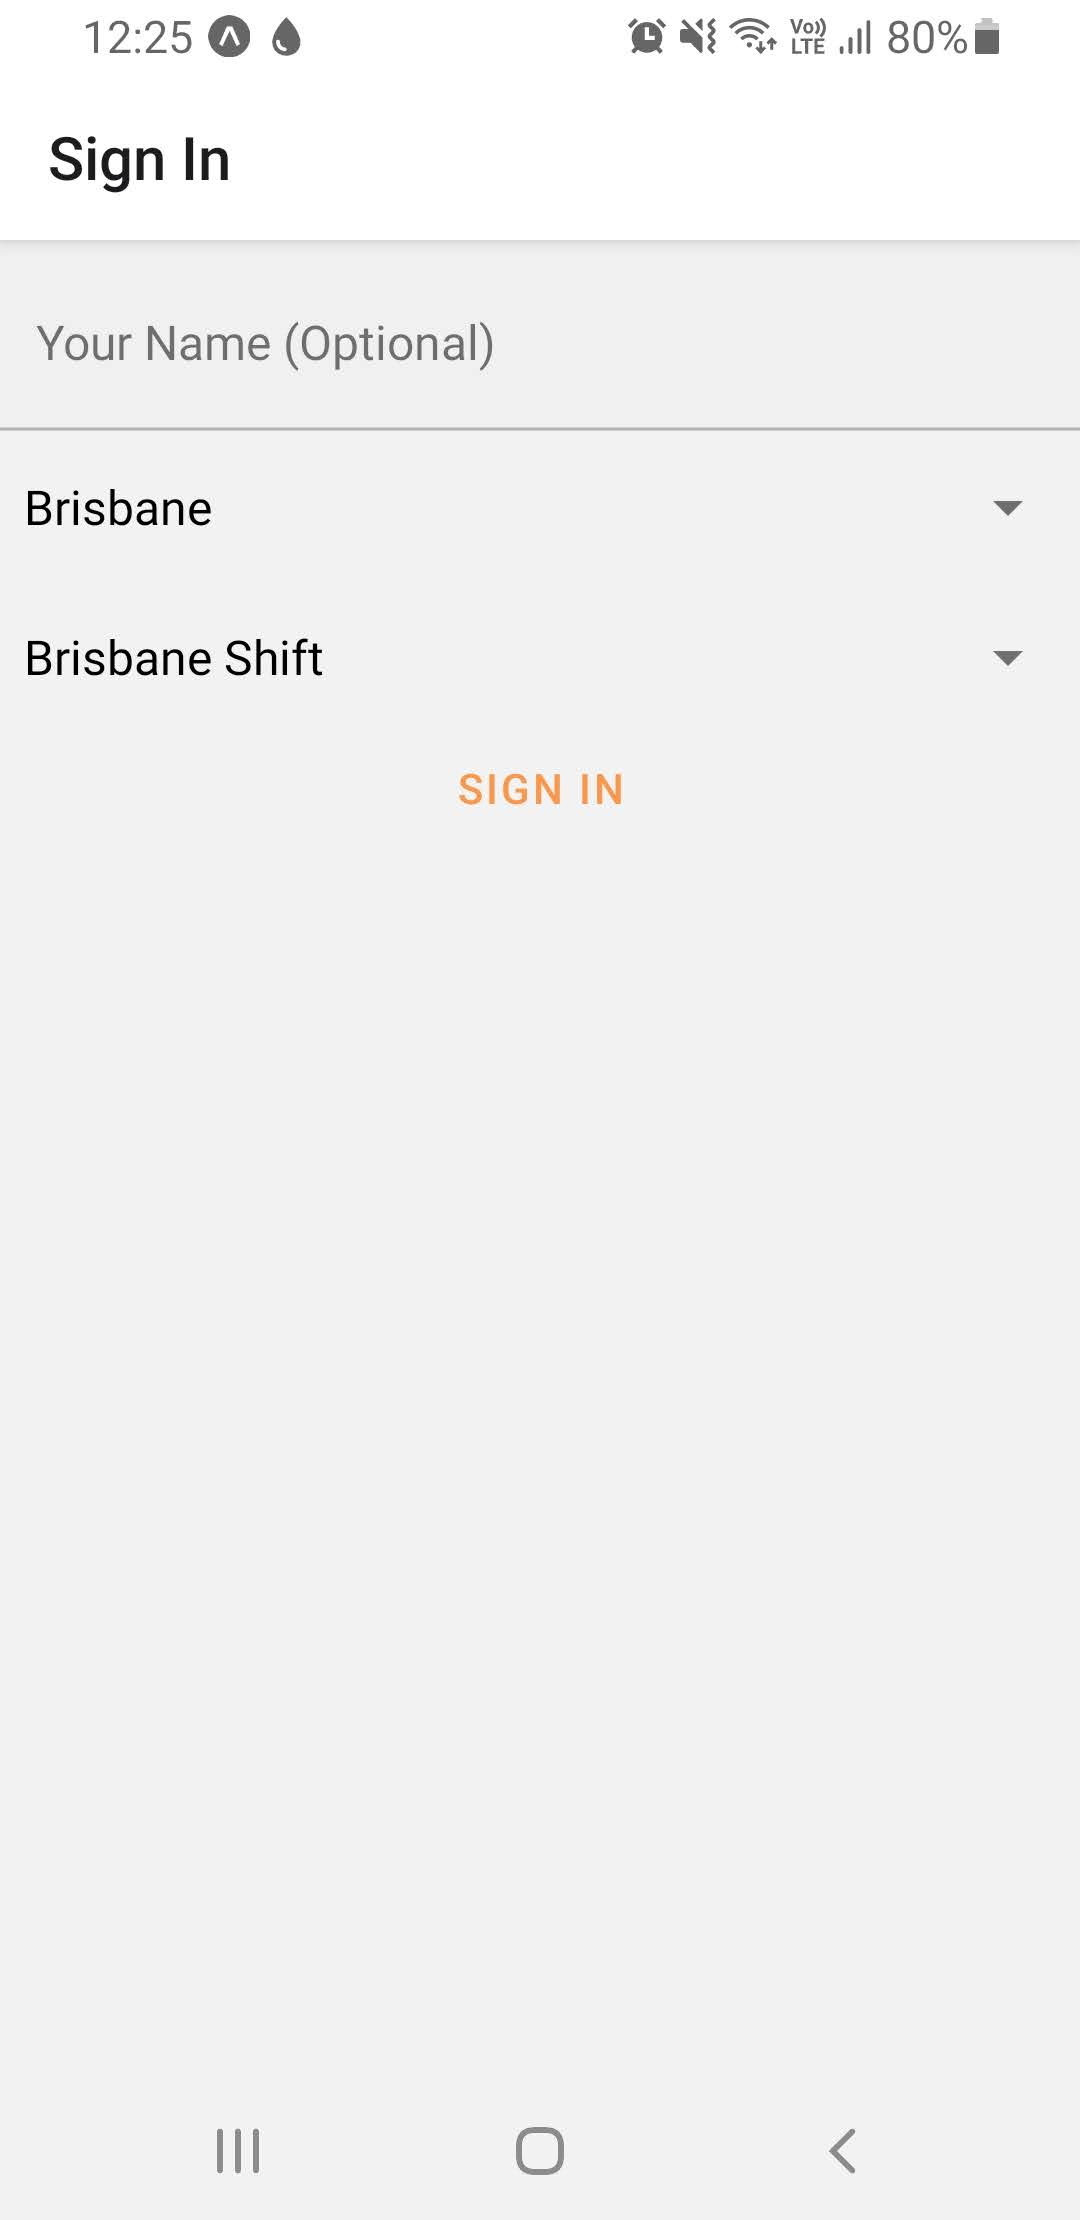
\includegraphics[scale=0.15]{assets/designs/screens/login.jpg}
    \caption{\centering{Login: Basic design, pushed to the top to leave room for a large tablet keyboard.}}
\end{figure}

\begin{figure}[ht!]
    \centering
    
\includegraphics[scale=0.25]{assets/designs/screens/home.jpg}
    \caption{\centering{Home: Intended to make it immediately apparent what the two core functions of the application are.}}
\end{figure}

\begin{figure}[ht!]
    \centering
    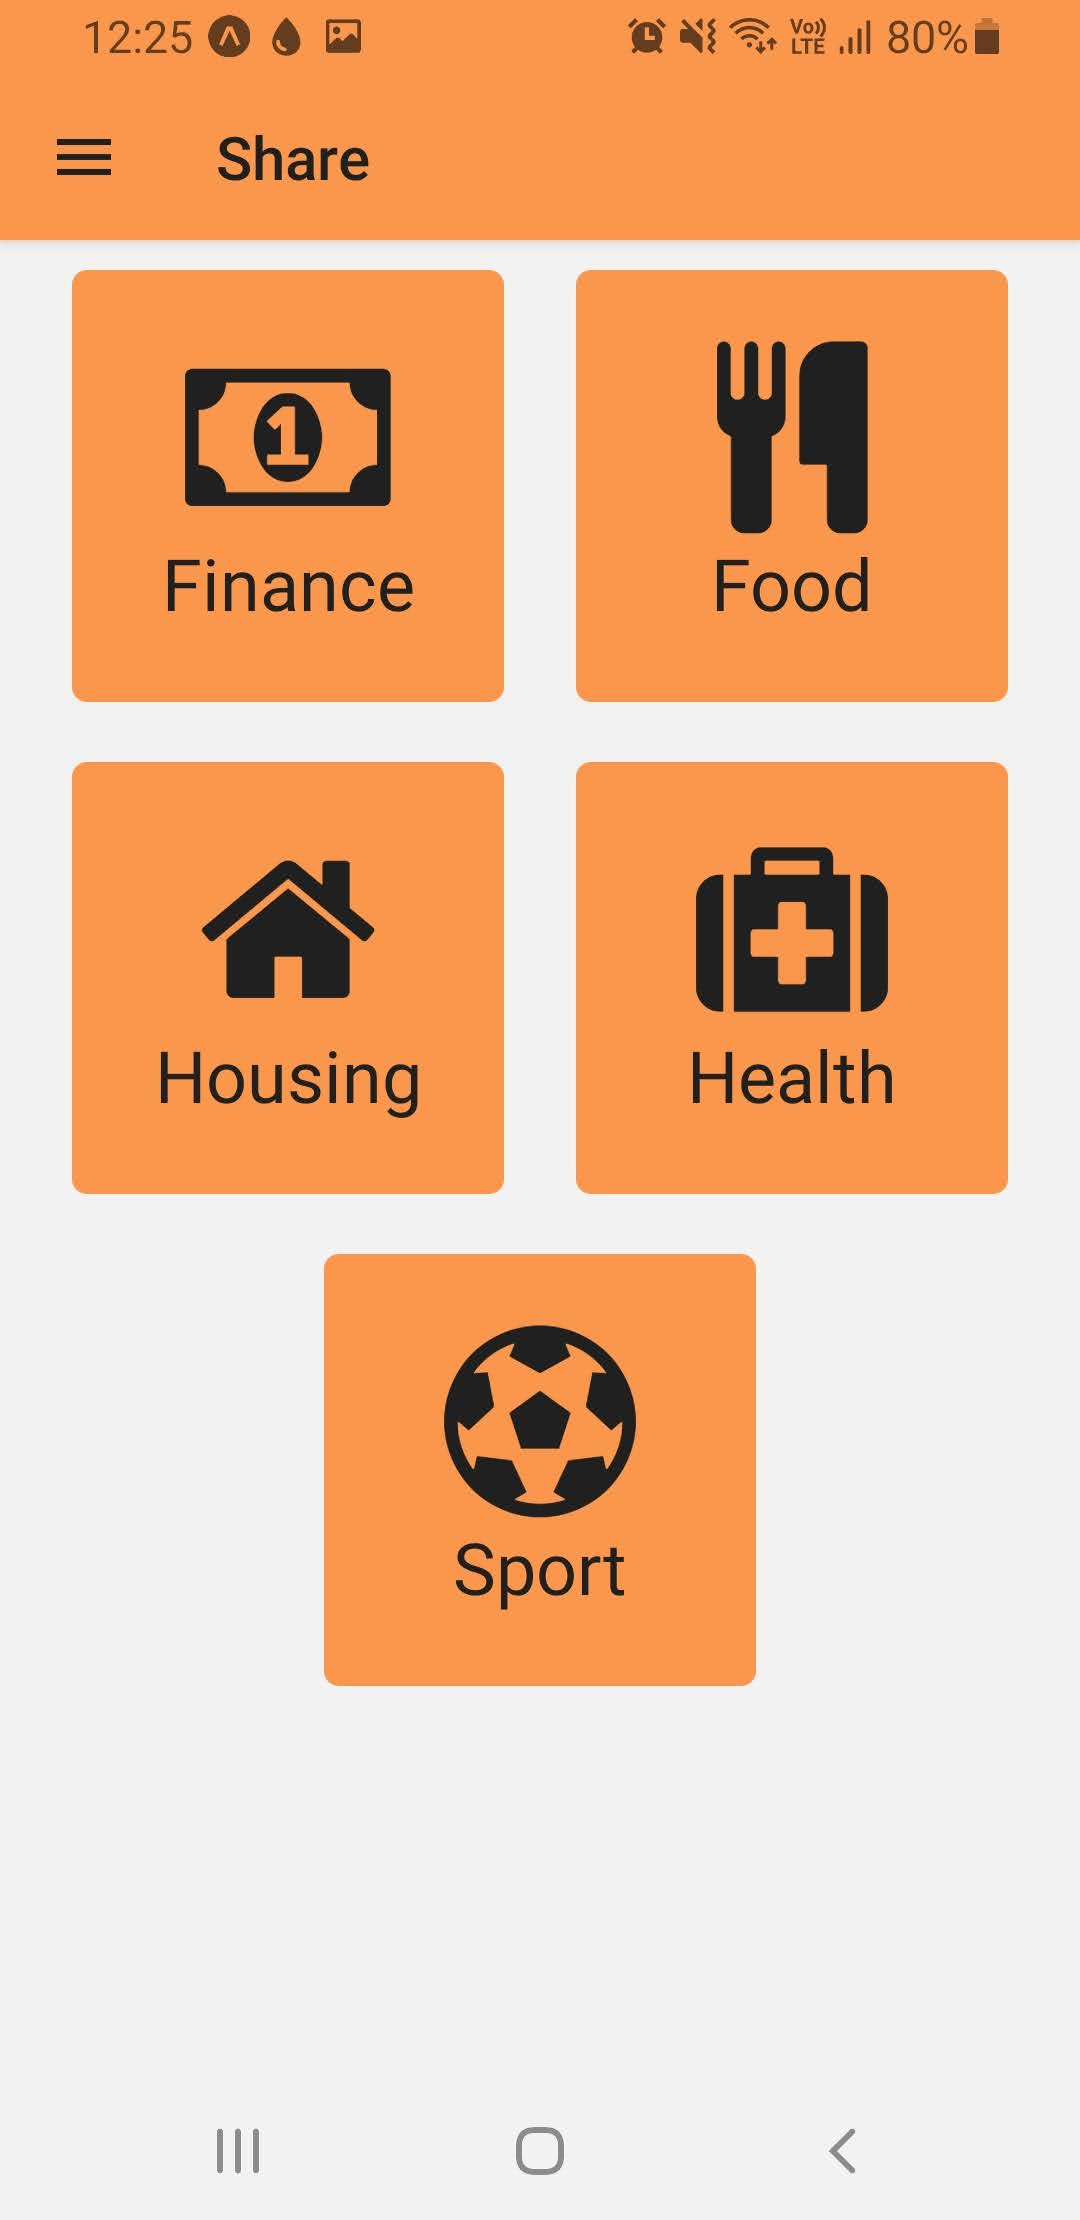
\includegraphics[scale=0.25]{assets/designs/screens/categories.jpg}
    \caption{\centering{Categories: A category selection screen to help prompt potential stories, as well as allow for targetted listening. The categories shown here are not indicative of those used on the final prototype.}}
\end{figure}

\begin{figure}[ht!]
    \centering
    
\includegraphics[scale=0.25]{assets/designs/screens/share.jpg}
    \caption{\centering{Share: A screen for capturing audio recordings, similar in design to most voice memo applications that users may have familiarity with.}}
\end{figure}

\begin{figure}[ht!]
    \centering
    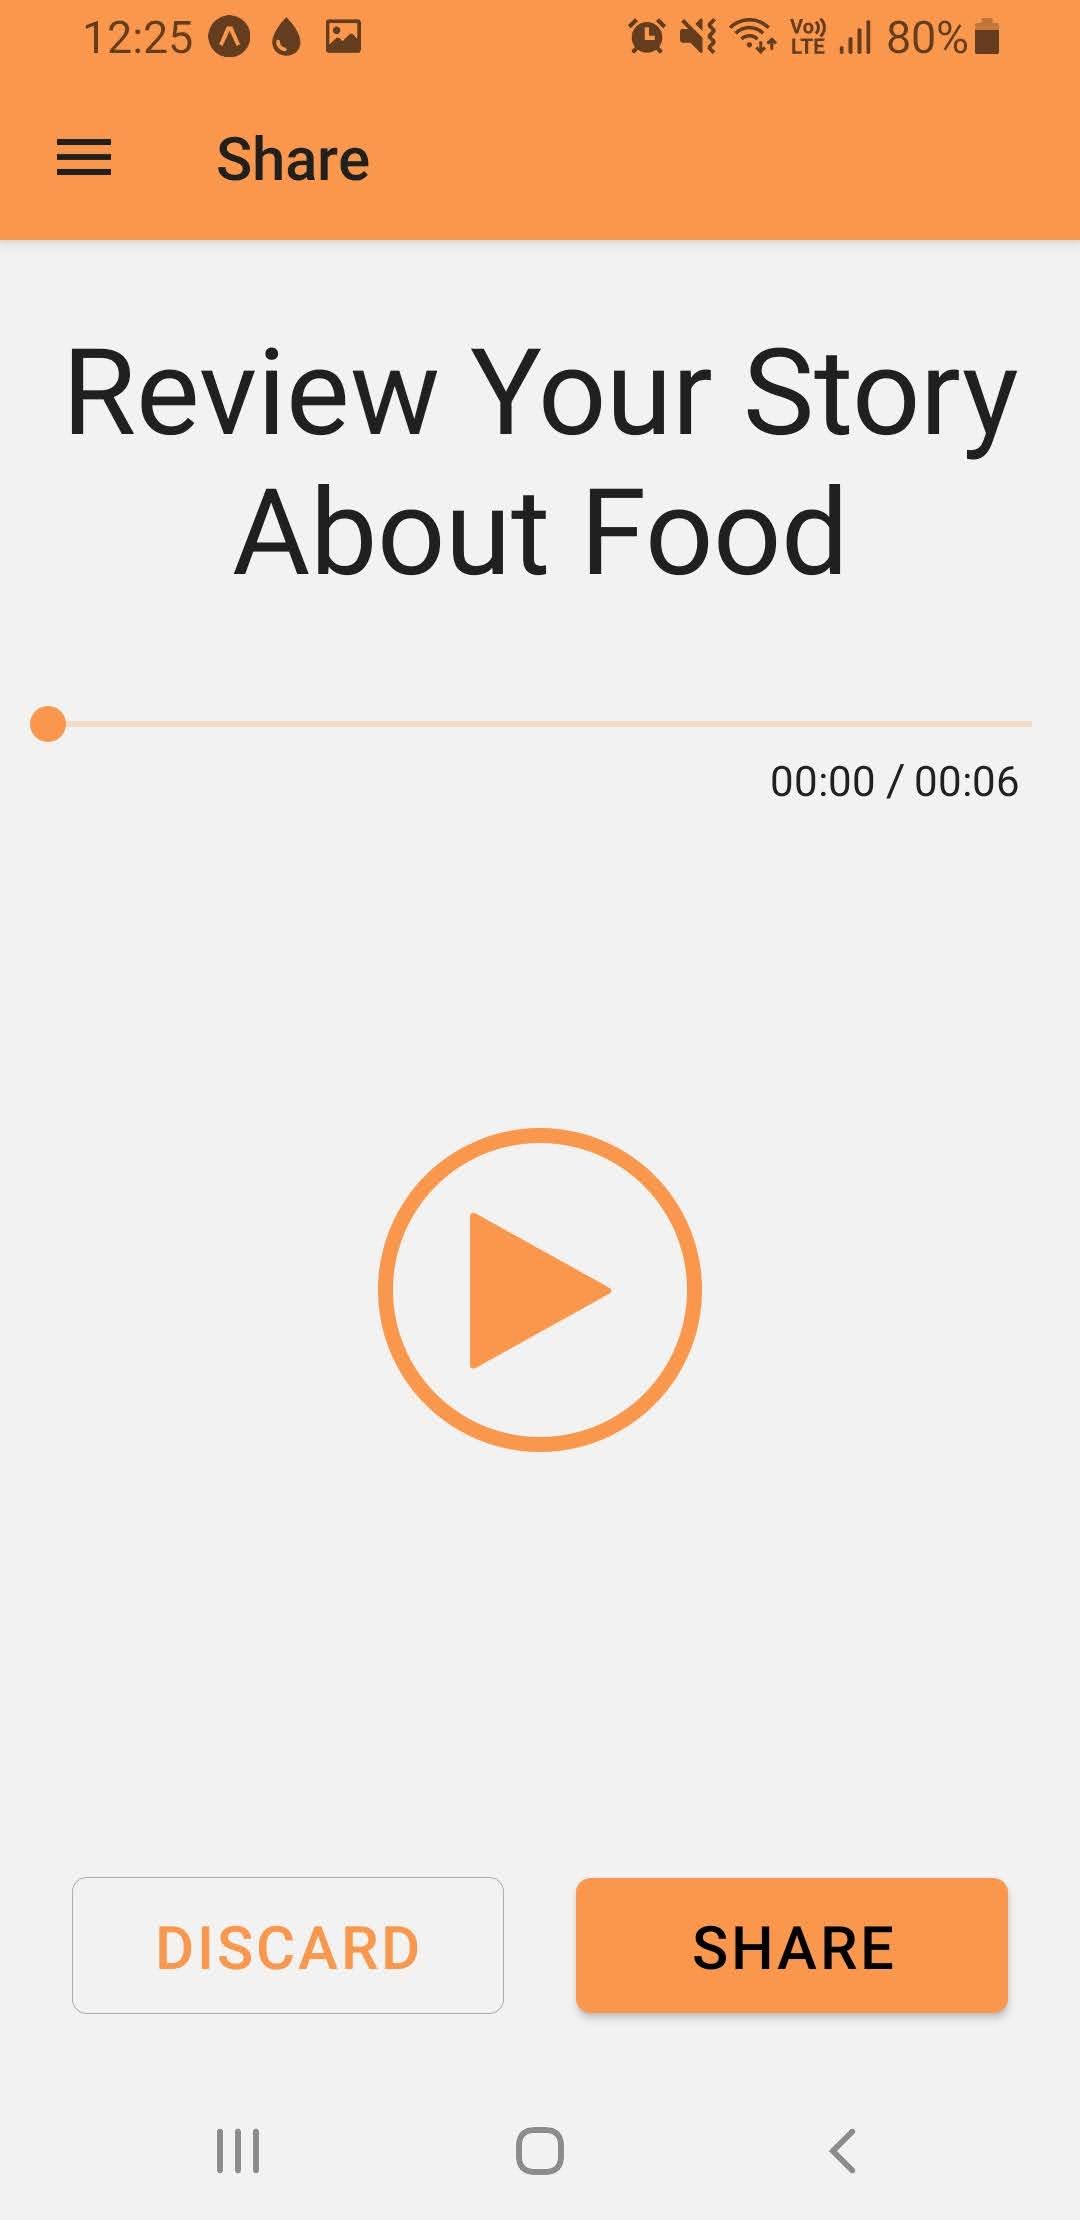
\includegraphics[scale=0.25]{assets/designs/screens/review.jpg}
    \caption{\centering{Review: A screen to provide the user with the ability to review their story before sharing}}
\end{figure}

\begin{figure}[ht!]
    \centering
    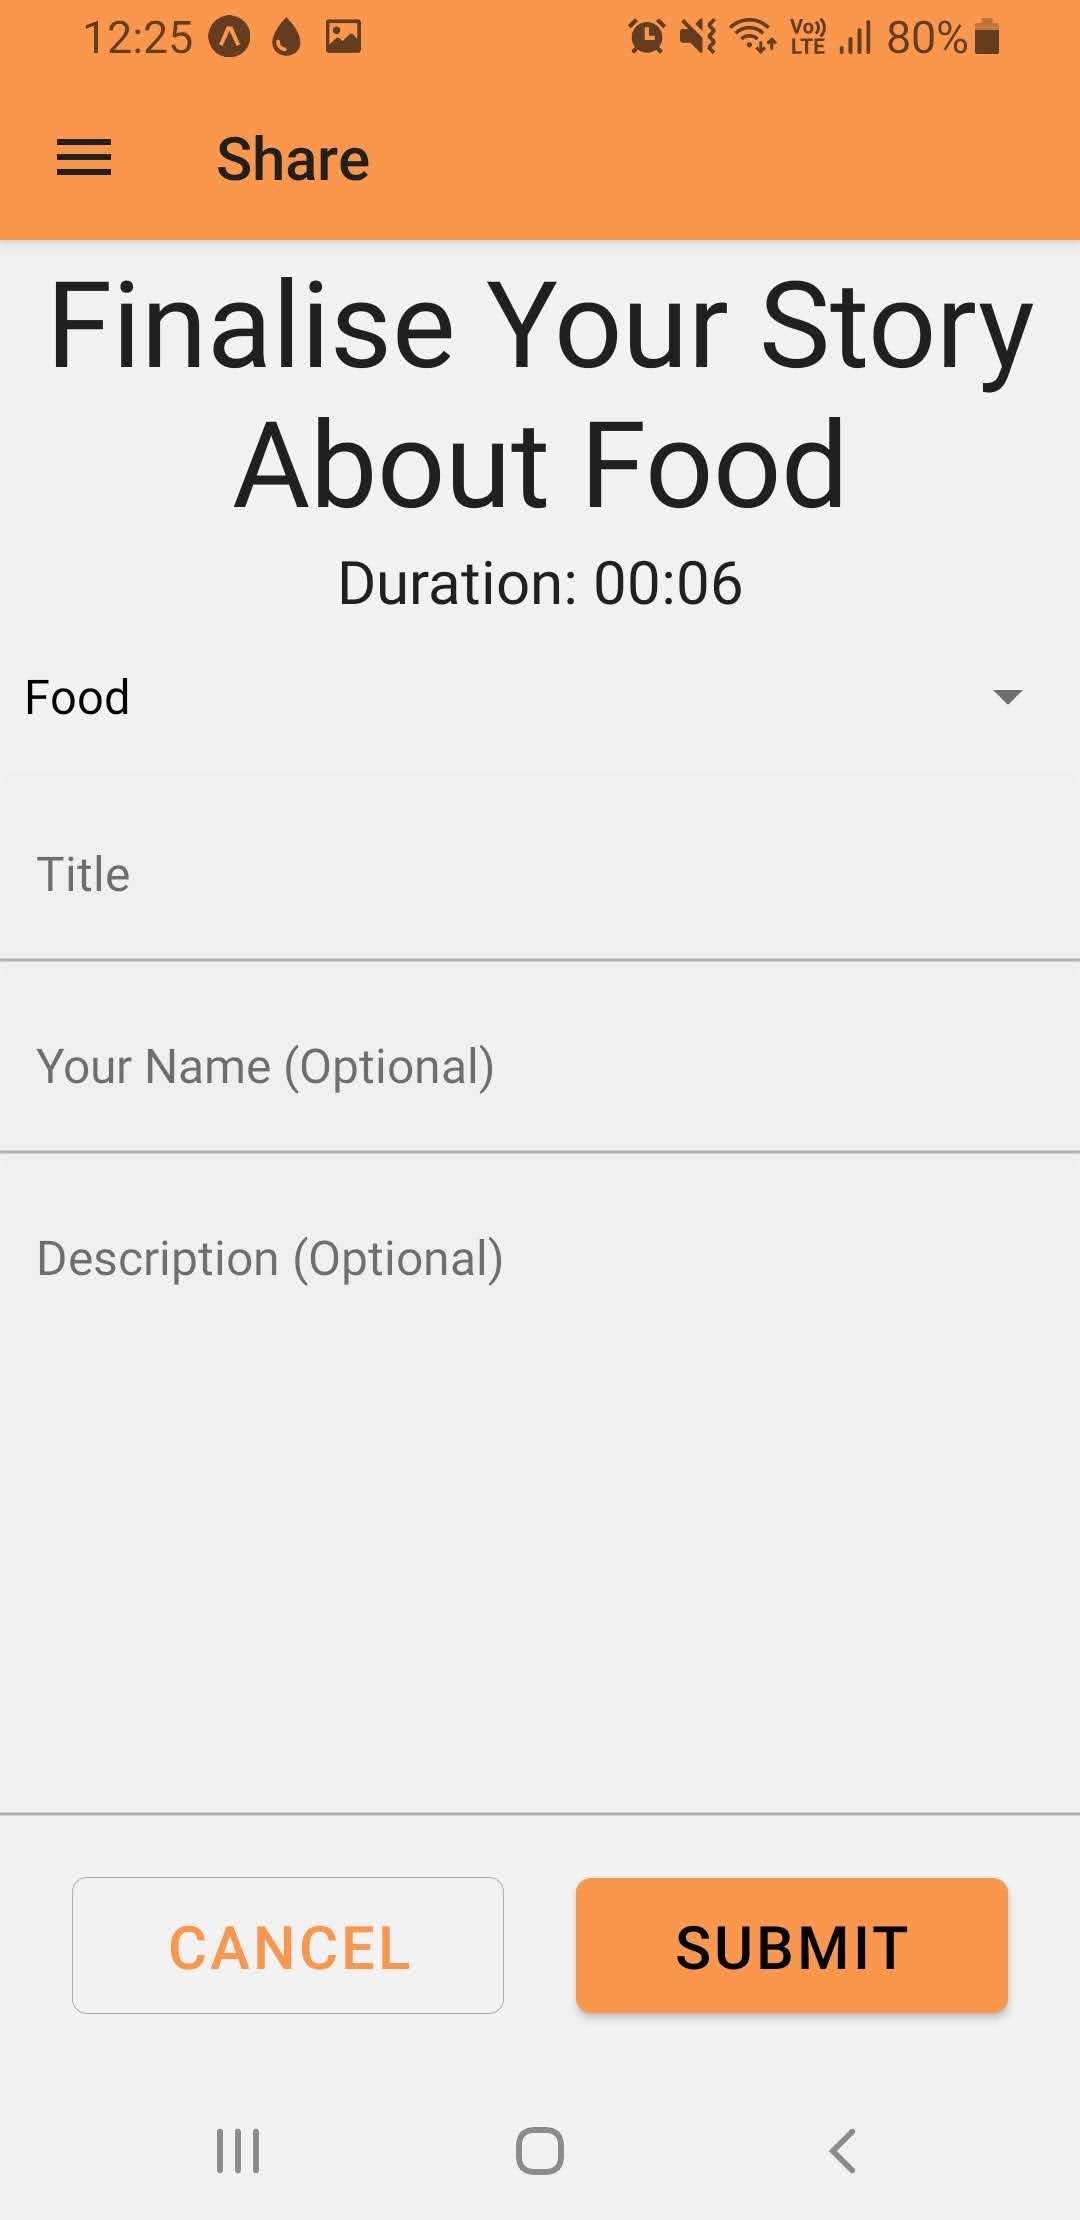
\includegraphics[scale=0.25]{assets/designs/screens/finalise.jpg}
    \caption{\centering{Finalise: Giving the user the opportunity to provide supporting textual information alongside their story, as well as to review their previously provided information such as name and category.}}
\end{figure}

\begin{figure}[ht!]
    \centering
    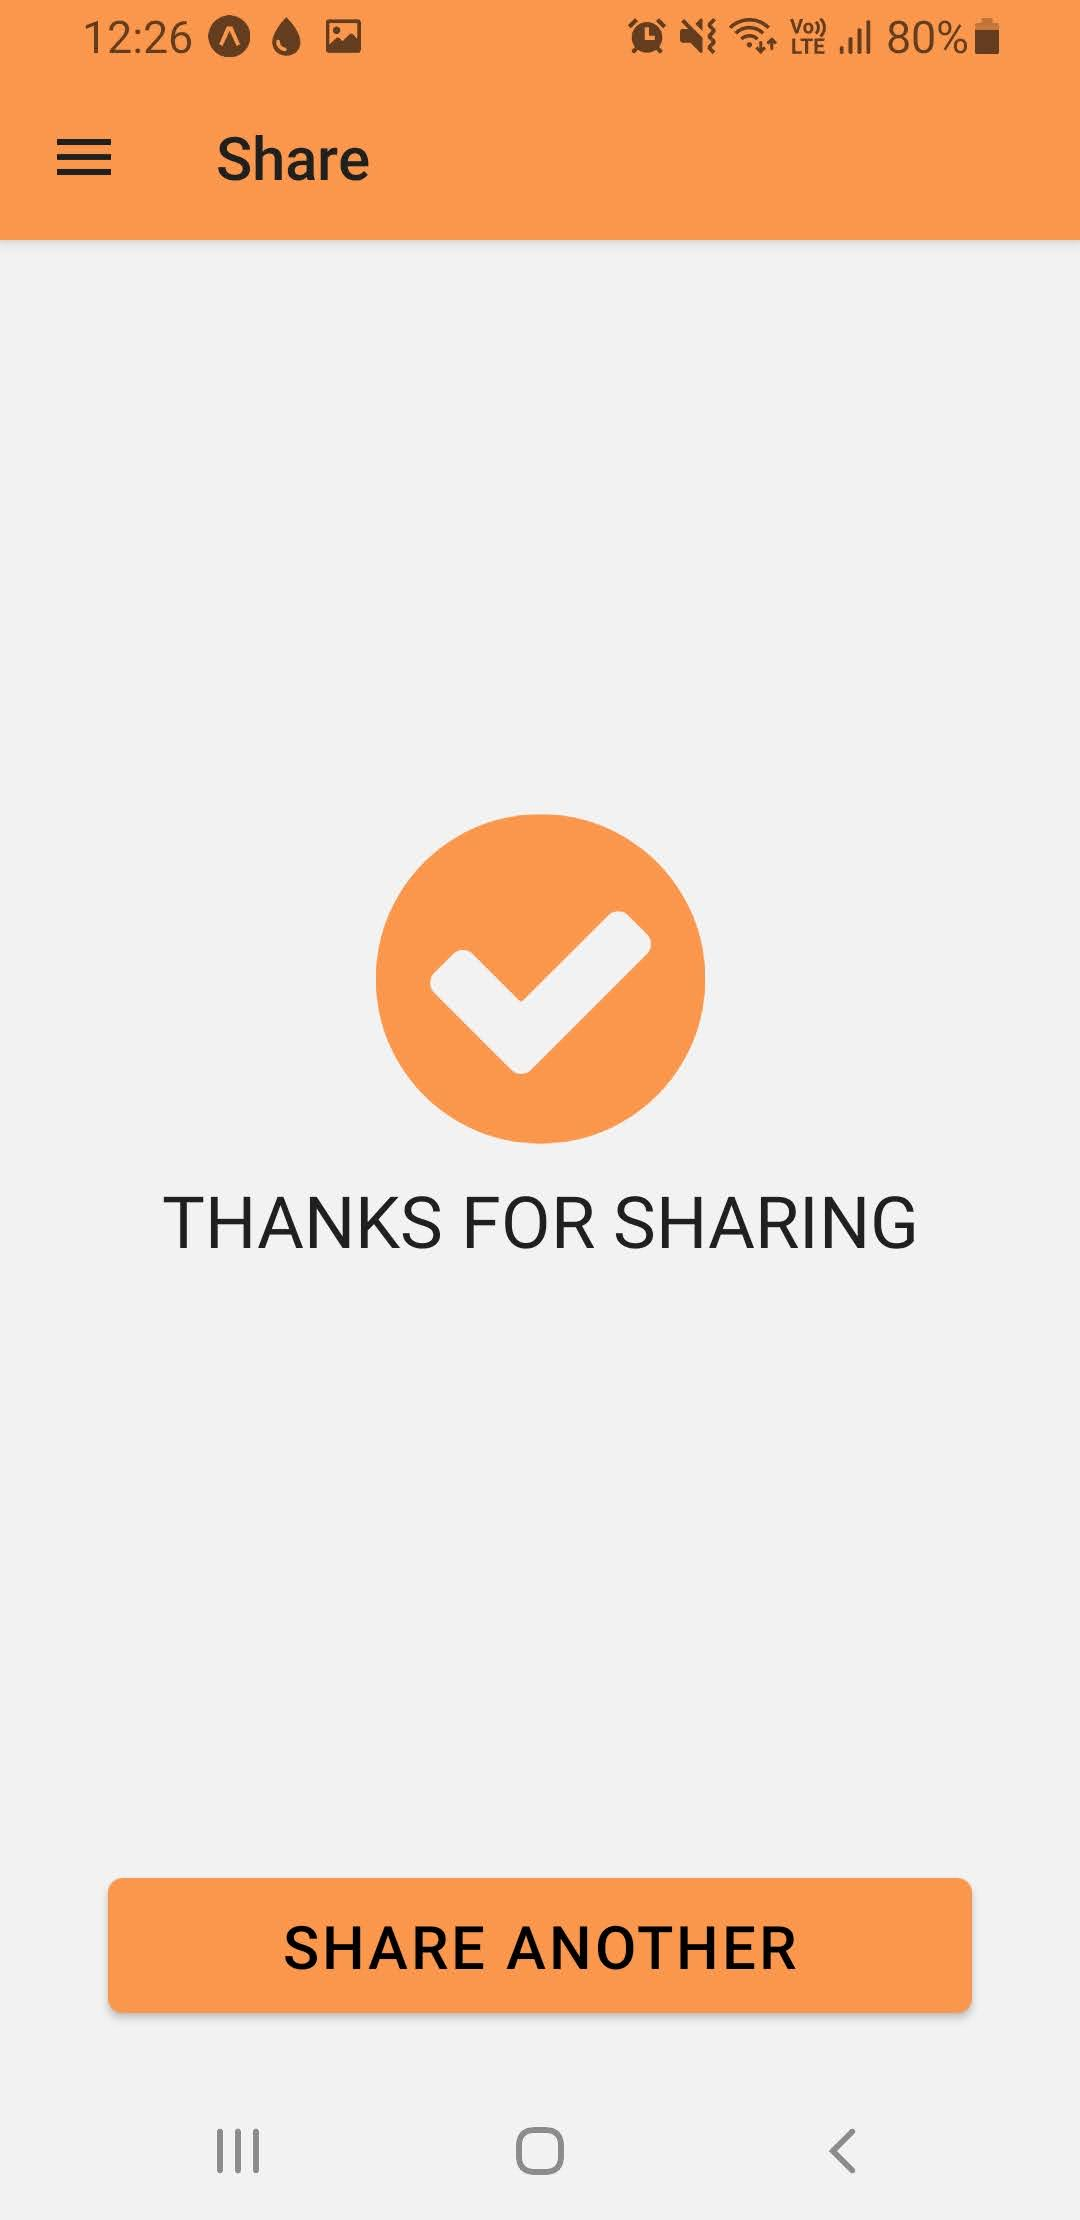
\includegraphics[scale=0.25]{assets/designs/screens/thanks.jpg}
    \caption{\centering{Thanks: A thank you screen for user's who share their story, also a clear indicator of a successful share.}}
\end{figure}

\begin{figure}[ht!]
    \centering
    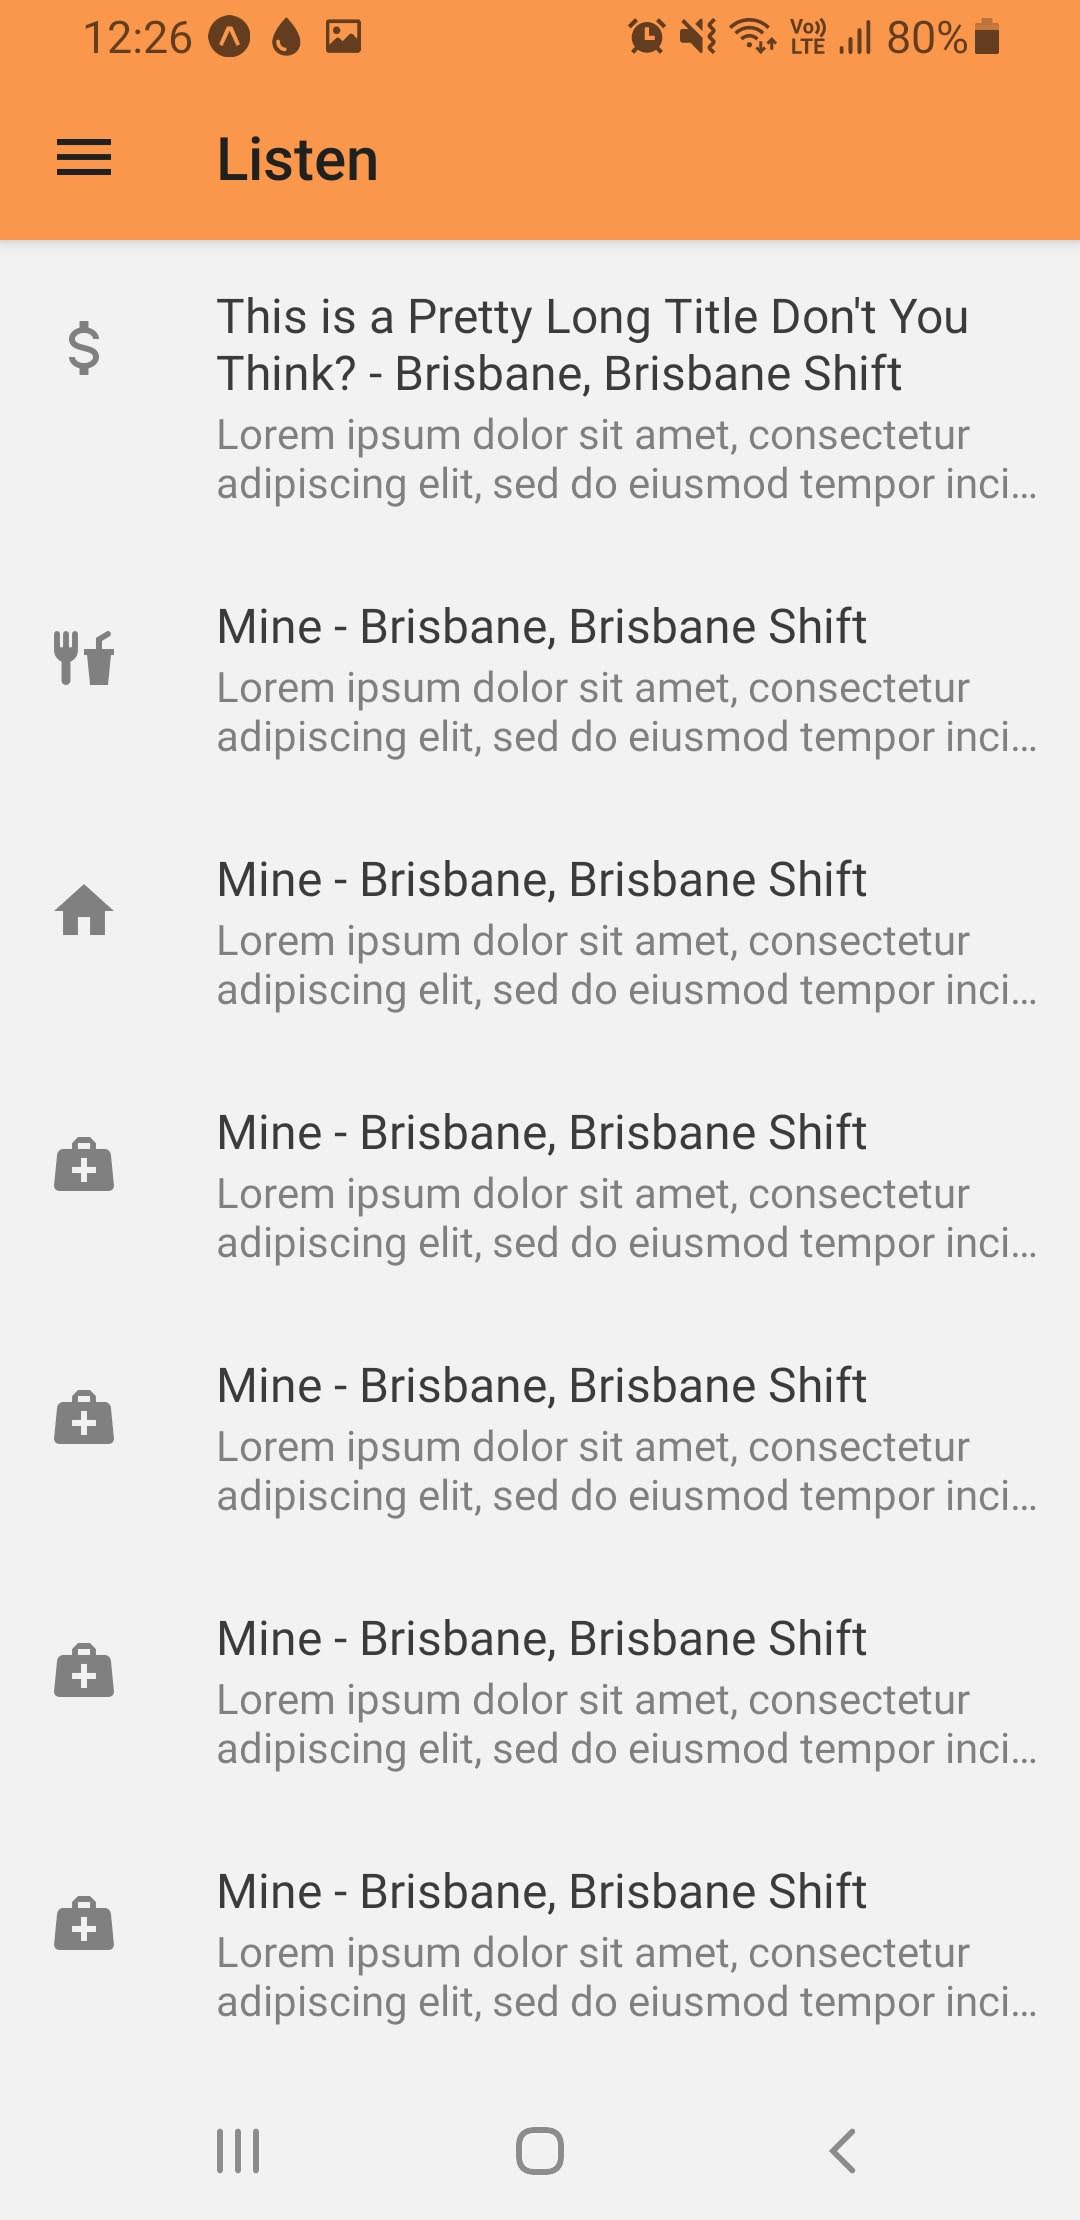
\includegraphics[scale=0.25]{assets/designs/screens/browse.jpg}
    \caption{\centering{Browse: An endlessly scrolling catalogue of previously shared stories, utilising the categories to provide informative metadata at a glance.}}
\end{figure}

\begin{figure}[ht!]
    \centering
    
\includegraphics[scale=0.25]{assets/designs/screens/listen.jpg}
    \caption{\centering{Listen: A simple screen for listening to stories shared by other users, note that the functionality to comment on and heart stories was also added to this screen prior to testing.}}
\end{figure}